\documentclass{article}
\usepackage[utf8]{inputenc}
\usepackage[russian]{babel}
\usepackage{multicol}
\usepackage[14pt]{extsizes}
\usepackage[left=5mm, top=1mm, right=5mm, bottom=0mm]{geometry}
\usepackage{graphicx}
\usepackage[document]{ragged2e}


\setlength\columnsep{50pt}
\begin{document}


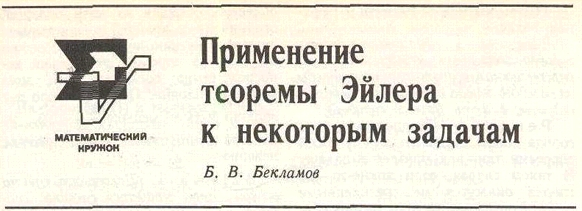
\includegraphics [width=207mm,height=70mm]{pic1}


\begin{multicols}{2}
\begin{small}
\begin{justify}

\parindent15pt
В этой статье мы предлагаем чи-\linebreak
тателям несколько задач, в решении\linebreak
которых центральную роль ишрает\linebreak
теорема Эйлера. Уделяя основное\linebreak
внимание задачам, мы не доказываем\linebreak
здесь эту теорему, а приводим лищь\linebreak
ее формулировку.Доказательство тео-\linebreak
ремы Эйлера, как и более общие фор-\linebreak
мулировки этой теоремы, можно найти\linebreak
в книгах "Что такое математика?"\linebreak
Куранта и Роббинса и "Наглядная\linebreak
геометрия" Гильберта и Кон-Фоссена.

\parindent15pt
Прежде чем формулировать теоре-\linebreak
му Эйлера, договоримся, что линию\linebreak
с концами в двух данных точках мы\linebreak
будем называть дугой, соединяющей\linebreak
эти точки, в том случае, если эту\linebreak
линию можно пройти, не побывав ни\linebreak
в одной из ее точек дважды.

\parindent15pt
Т е о р е м а   Э й л е р а. Пусть\linebreak
на плоскости задано m точек и n по-\linebreak
парно непересекающихся дуг, каждая\linebreak
из которых соединяет какие-либо две\linebreak
данные точки и не проходит черех\linebreak
остальние m - 2 точки, и пусть эти\linebreak


\parindent0pt
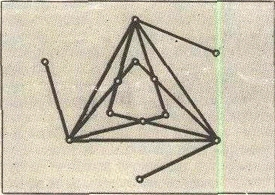
\includegraphics[width=95mm,height=62mm]{picture/ris2.jpg}


дуги делят плоскость на L облостей.\linebreak
Если из каждой данной точки в любую\linebreak
из остальных можно попасть,двишаясь\linebreak
по этим другам, то\linebreak

\parindent60pt
m - n + L = 2

\parindent15pt
$\Delta A$ = - $q_2$($\varphi$$_2$ - $\varphi$$_1$) = -$q_2$$q_1$\\

\parindent60pt
\indent ($\frac{1}{r + r} - \frac{1}{\Delta r}$) = $\frac{q_1 q_2 \Delta r}{r^2 + r \Delta r}$. \\

\parindent20pt
\indent Так как $\Delta r$ мало, то $r^2$ $\gg$ r$\Delta$r и \\

\parindent45pt
\indent $\Delta A$ = $F \Delta r$ = $\frac{q_1 q_2}{r^2} \Delta r .$ 
\linebreak

\parindent15pt
В некоторых задачах совокуп-\linebreak
ность, состоящих из нескольких то-\linebreak
чек и соединяющих из нескольких то-\linebreak
чек и соединяющих их попарно не-\linebreak
пересекающихся дуг, мы называем\linebreak
картой; при этом точки из этой сово-\linebreak
купности мы называем вершинами,\linebreak
а облости, на которые дуги делят\linebreak
плоскости, - старнами.

\parindent0pt

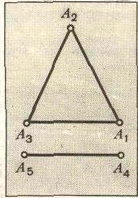
\includegraphics[scale=1.25]{picture/3.jpg}
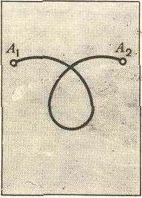
\includegraphics[scale=1.25]{picture/4.jpg}

\end{justify}
\end{small}
\end{multicols}
\end{document}